\documentclass[12pt, a4paper]{article}

\usepackage[utf8]{inputenc}
\usepackage{graphicx} % to embed images
\usepackage{rotating}
\usepackage{hyperref} % to link the table of contents
\usepackage{subcaption} %complex images
\usepackage{placeins} %floating
\usepackage{pdflscape} %to allow single pages in landscape mode
\usepackage[top=1.25in, bottom=1.25in, left=1in, right=1in]{geometry}
\usepackage{verbatim} % include raw text file (for Alloy)
\usepackage[ruled, vlined]{algorithm2e} % algorithms
\usepackage[export]{adjustbox}
\usepackage{multirow}
\usepackage{enumitem}

\newcommand{\paragraphnewline}[1]{\paragraph{#1}\mbox{}\\}


\title{Integration Test Plan Document}
\date{2017-01-15}
\author{
	Patricia Abbud
	\and
	Maddalena Andreoli Andreoni
	\and
	Paolo Cudrano
}

\begin{document}
	%%% titlepage %%%
	\begin{titlepage}
		\centering
		
\includegraphics[width=5cm]{img/polimi_logo.png} % also works with logo.pdf
		\vfill
		{\bfseries\Large
			PowerEnJoy\\
			Integration Test Plan Document\\
			\vskip4cm
			Patricia Abbud\\
			Maddalena Andreoli Andreoni\\
			Paolo Cudrano\\
		}
		\vfill
		\vfill
	\end{titlepage}

	%%% table of contents %%%
	\tableofcontents
	\newpage

	\section{Introduction}
		\subsection{Purpose}
This Design Document describes the architecture and design choices for \textit{PowerEnJoy}'s system the team is to develop. The document will be divided in five main chapters (aside from the introduction and appendixes): the \textbf{Architectural Design} chapter will describe in detail our system, the architectural choices we made and its design. It will make use of UML diagrams as well as text descriptions, going from a high-level view to a more deep and in-detail analysis. The \textbf{Algorithm Design} will focus on the most relevant algorithmic parts of the system, mainly related to the \textit{money saving option}: it will contain a short description of each algorithm as well as the algorithm itself. 
The \textbf{User Interface Design} section will provide an overview of the user interfaces of the system. Since some of it have already been described in the RASD document, this section will only contain the remaining ones. 
Finally, the \textbf{Requirements Traceability} will map the requirements defined in the RASD document to the design elements defined in this document.
Every step in the decision process will be documented and explained.

\subsection{Scope}
The goal of this project is to create \textit{ex novo} a system for the car-sharing service \textit{PowerEnJoy}. This system will provide users throughout the city an easy and user-friendly way to reserve and drive electric cars, and also to interact with the company's operators and administrators in the eventuality of a break down or an accident.

\subsection{Definitions, acronyms, abbreviations}
% TODO

\subsection{Reference documents}
% TODO

\subsection{Document structure}
% TODO

	\newpage
	\section{Integration strategy}
		\subsection{Entry criteria}
\label{sec:entry_criteria}
	In order for the integration process to be performed, a set of preconditions must be met. In particular:
	\begin{description}
		\item[Database] The complete schema provided by the DD must be implemented and tested. The database access system must be at 100\% of its development, and the database must be fully accessible.
		\item[Application logic] Referencing to the components designed in section \textit{2.2 - Component view} of the DD, they must all be unit tested before their integration starts. In addition, their development completion ratio must be so that all the functionalities needed for the integration are already fully developed. 
		% TODO? This approximately translates in the following completion thresholds: <list>
	\end{description}
	Once begun, the integration testing follows and guides the development, as explained in \autoref{sec:integration_testing_strategy}. % FIXME check correctness and add link

\subsection{Elements to be integrated}
\label{sec:elements_to_be_integrated}
	As explained in the DD, the three layers in which the system is divided are characterized as follows.
	\begin{description}
		\item[Data] A database holds and gives access to all the data needed by the application. As anticipated in \autoref{sec:entry_criteria}, this layer does not participate actively in the integration process. Indeed, since its development isn't particularly demanding in terms of resources, it is assumed to be already completed once the integration begins. This way, every logic component will be able to access the data layer during the unit testing phase, and integrate with it as a prerequisite for the proper integration phase.
		\item[Application logic] The components on which most of the integration effort will be spent are those intensively described in section \textit{2.2 - Component view} of the DD. These represent the main software components of the system and are responsible to provide the functionalities required by it. In particular, the integration will proceed on two different abstraction layers (one considering only macro-components, the other considering the internal interactions among subcomponents), and a particular attention will be paid for the subcomponents residing on different machines (e.g.: server and client). For this last reason, when dealing with subcomponents we will graphically differentiate them when they are deployed on the server (their diagram will be colored light blue) and when they are deployed on a client (light yellow).
		\item[View] The view layer won't be affected by the integration process. It will be unit tested during its development, and since its instances are each connected only with a single application logic component, their integration will be straightforward and won't need a delicate testing. The view functioning will be however tested during the more general \textit{system testing} phase. % FIXME ok? Old notes: view unit tested, integration done at the end??, but then why not tested? / main focus on application logic, view just unit tested because dumbly integrated to the rest.
	\end{description}
	In this analysis, the website, for its simple and self-contained nature, will not be taken into account as it will not need an integration phase, jumping directly to the system testing phase.	\newline

	As a result, the set of macro-components to be considered for the integration testing becomes definite. Following are enlisted the macro-components on which the integration will be performed (at an internal-level first, and at a system-level after):
	\begin{itemize}
		\item \textbf{User Location Handler}
		\item \textbf{Operator Location Handler}
		\item \textbf{Car Location Handler}
		\item \textbf{User Management server-side} with subcomponents: Profile Manager, License Manager
		\item \textbf{User Management client-side} with subcomponent: User Handler
		\item \textbf{Car Manager}
		\item \textbf{Access Manager}
		\item \textbf{Parking Manager}
		\item \textbf{Car Employment Manager}
		\item \textbf{Maintenance Manager client-side} with subcomponent: Operator Handler
		\item \textbf{Maintenance Manager server-side} with subcomponents: Emergency Report Handler, Report Status Handler, Dispatch Manager
		\item \textbf{Money Saving Option Manager}
		\item \textbf{Backend Manager client-side} with subcomponent: Admin Handler
		\item \textbf{Backend Manager server-side} with subcomponent: Backend Manager
		\item \textbf{Payment Manager}
	\end{itemize}
	

\subsection{Integration testing strategy}
\label{sec:integration_testing_strategy}
	The integration of the system will be guided by a bottom-up approach. This strictly comes from an analysis of the dependency structure of the components diagram provided in the DD, restructured in \autoref{fig:dependency_tree_high} and \autoref{fig:dependency_tree_complete} to better highlight the key modules and their connections.
	\begin{figure}[h]
		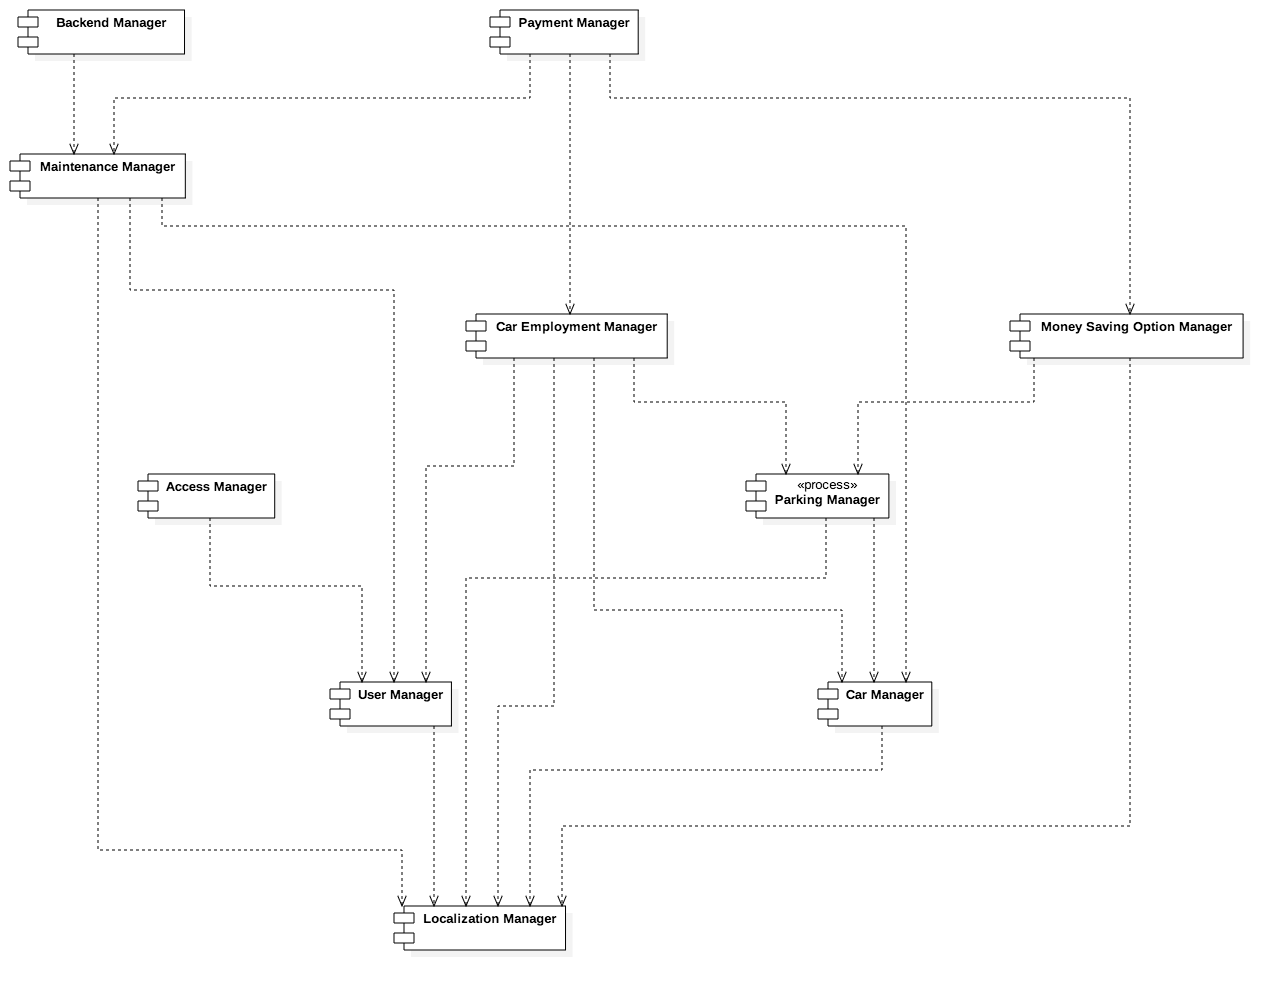
\includegraphics[width=\textwidth, center]{img/integration_strategy/high_level_unravelled.png}
		\caption{Dependency tree of components: high level view.}
		\label{fig:dependency_tree_high}
	\end{figure}
	\begin{figure}[h]
		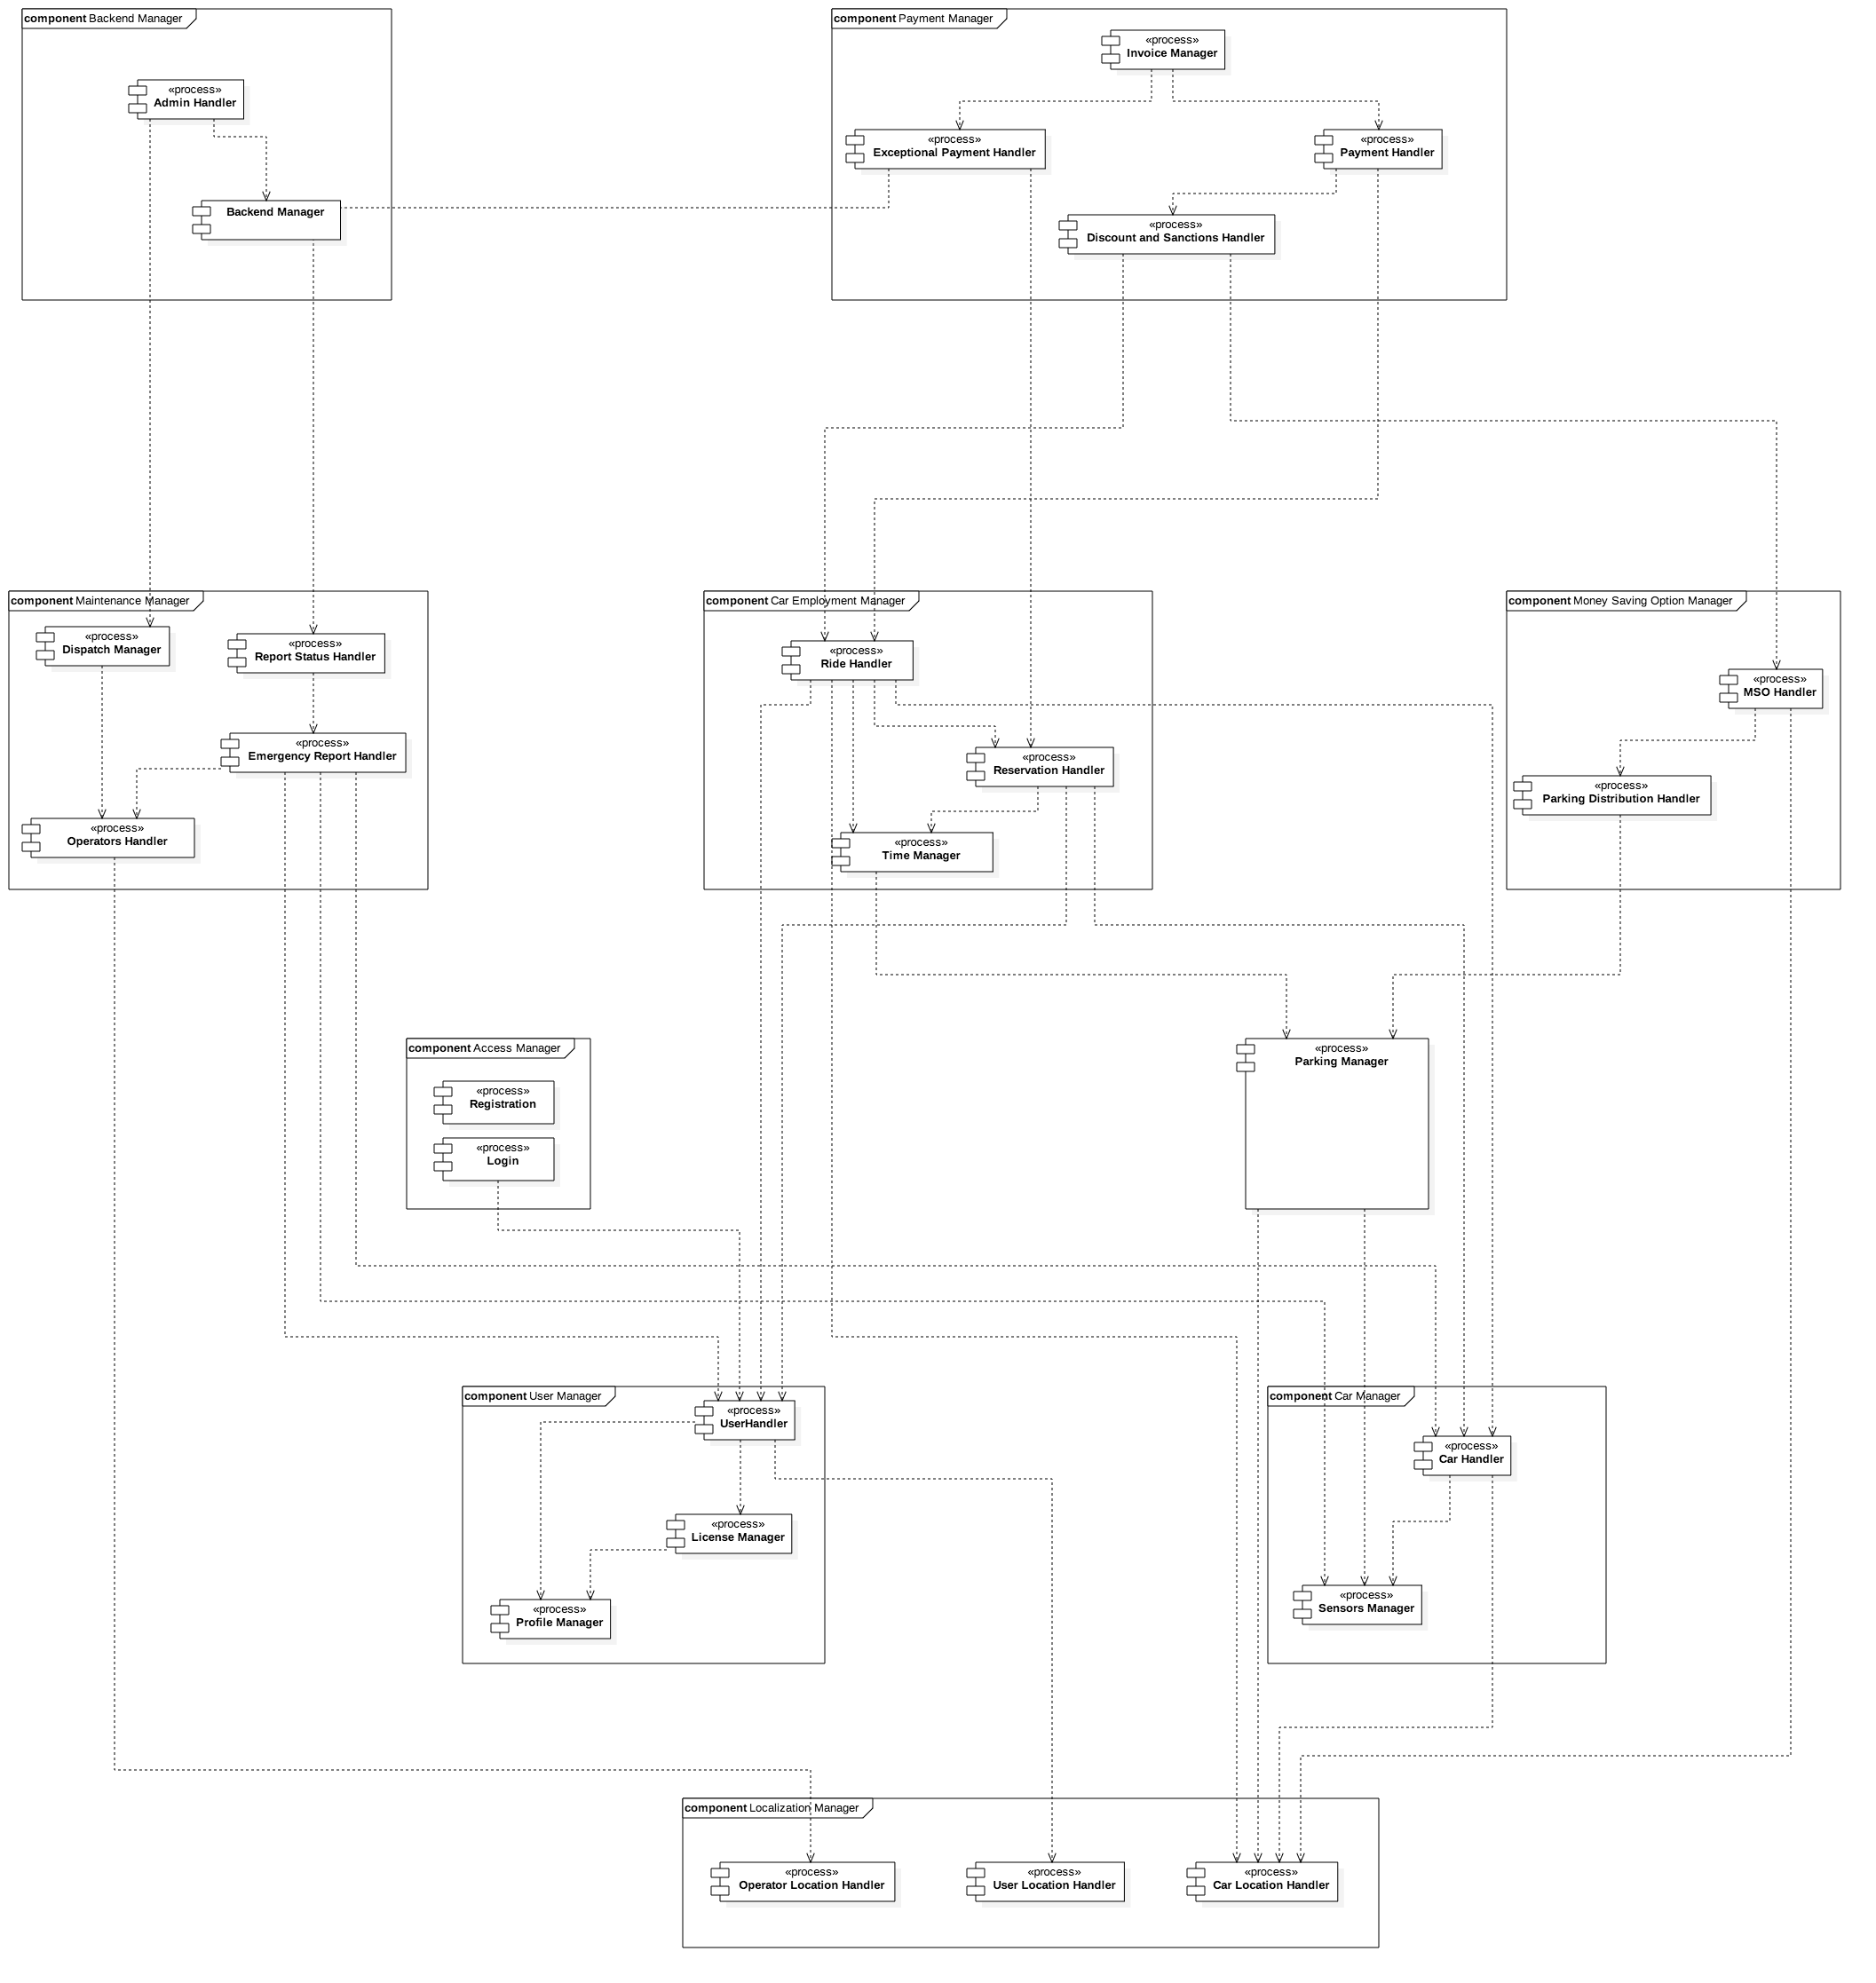
\includegraphics[width=\textwidth, center]{img/integration_strategy/complete_unravelled.png}
		\caption{Dependency tree of components: complete system.}
		\label{fig:dependency_tree_complete}
	\end{figure}

	This strategy allows for a close interaction between the development phase and the proper testing phase, with a benefit for the quality of the software-to-be as well as for the project management. The goal set with this choice is to make development and testing actually going in parallel during standard operating periods. %% a regime, come si dice!!
	% TODO sth more about it?
	The approach used to integrate the different subcomponents inside a single macro-component is instead selected according to its level of criticality; in particular, the choice revolves around a "nested" bottom-up approach on one hand, and a more complex critical-first approach on the other.
	A criticality analysis underlines the following critical macro-components.
	\begin{itemize}
		\item \textbf{Car Manager.} The integration of the car system software with the underlying hardware and the sensors it is managing involves a moderate number of uncontrollable variables and introduces with them a certain amount of risk. In fact, it is the only point of contact with the actual car, thus becoming the contact point between two rather complex systems.
		\item \textbf{Money Saving Option Manager.} Even if not crucial for the basic functioning of the system, this macro-component is responsible for a large amount of computations, carried on by means of complex algorithms. These must be tested as soon as possible in order to obtain the desired results. In addition, the main algorithm provided by the \textit{Parking Distribution Handler} is designed to be implemented with the not-so-common paradigm of fuzzy logic (see DD \textit{section 3}), and as any not-well-spread development tool, this may suffer for less stability and minor flaws, which must be discovered and managed as soon as possible.
		\item \textbf{Payment Manager.} The payment handling is known to be one of the most critical activities since it involves money transactions. In particular, since the system relies on an external company for the actual payment realizations, its most critical subcomponent is the Invoice Manager, responsible for the interactions with the external \textit{Payment Services Provider}.
	\end{itemize}
	As a result, when the said macro-components are to be developed, their internal integration will follow a critical-first approach. This increases the chances that any significant problem is found as soon as possible, and therefore should provide benefits in the project management (rescheduling of tasks, reallocation of resources, etc.) aside from the integration process itself.
	% TODO should say here which is the order for these? or in section 2.4?

	The rest of the macro-components, given their less risky nature, will be internally developed following a bottom-up strategy, where the subcomponents are considered all equally-critical and only the "need" dependencies will drive the process.
\FloatBarrier

\subsection{Sequence of component/function integration}
	% see assignment pdf for a non mandatory guide on the structure of this subsection
	% - image of the division bottom up, maybe just with macrocomponents, and explaination
	% - [before or after] details on the single integrations?
	In the present section, the general criteria outlined before are translated to the actual sequence of integration steps to follow in the development and testing of the system. Their presentation will be made exploiting two levels of detail, in a bottom-up fashion: \autoref{sec:software_integration_sequence} refers to the integration of the various subcomponents in the context of a particular macro-component, while \autoref{sec:subsystem_integration_sequence} increases the abstraction level, focusing on how the different macro-components will be assembled to form the whole system.

	\subsubsection{Software integration sequence}
	\label{sec:software_integration_sequence}
		% TODO
		% - paragraph for each subsystem (macro component) --> list of images and description (without separations) for the steps, from 2 subcomponents to the whole completed subsystem.
		\paragraphnewline{Localization Manager}
			This component does not require internal integration and will only function as an helper for other components.

		\paragraphnewline{User Manager}
			\begin{itemize}[label={},leftmargin=*,noitemsep,topsep=0pt]
				\item \textit{Internal integration strategy:} bottom-up.
				\item \textit{Integration order:}
					\begin{itemize}[noitemsep]
						\item Profile Manager
						\item License Manager
						\item User Handler
					\end{itemize}
			\end{itemize}
			\begin{figure}[h]
				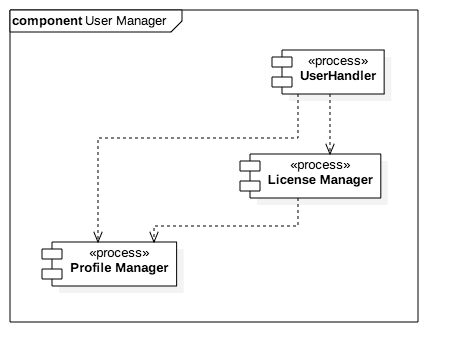
\includegraphics[width=250pt, center]{img/integration_strategy/subcomponents/user_manager.png}
			\end{figure}
		\FloatBarrier

		\paragraphnewline{Car Manager}
			\begin{itemize}[label={},leftmargin=*,noitemsep,topsep=0pt]
				\item \textit{Internal integration strategy:} critical-first.
				\item \textit{Integration order:}
					\begin{itemize}[noitemsep]
						\item Sensors Manager
						\item Car Handler
					\end{itemize}
				\item \textit{Notes: } The integration starts from the Sensors Manager because most of the criticality is related to the communication and management of the system's hardware, functionalities provided by it.
			\end{itemize}
			\begin{figure}[h]
				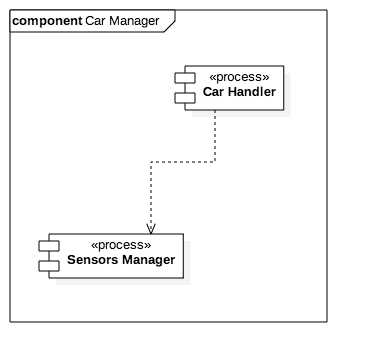
\includegraphics[width=250pt, center]{img/integration_strategy/subcomponents/car_manager.png}
			\end{figure}
		\FloatBarrier

		\paragraphnewline{Parking Manager}
			This component is atomic and thus does not require internal integration.

		\paragraphnewline{Access Manager}
			\begin{itemize}[label={},leftmargin=*,noitemsep,topsep=0pt]
				\item \textit{Internal integration strategy:} bottom-up.
				\item \textit{Integration order:}
					\begin{itemize}[noitemsep]
						\item Login
						\item Registration
					\end{itemize}
				\item \textit{Notes: } The integration starts from the Login because it must be subsequently integrated to the rest of the system, while Registration is independent from it.
			\end{itemize}
			\begin{figure}[h]
				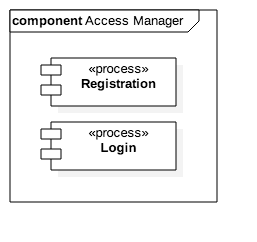
\includegraphics[width=150pt, center]{img/integration_strategy/subcomponents/access_manager.png}
			\end{figure}
		\FloatBarrier

		\paragraphnewline{Car Employment Manager}
			\begin{itemize}[label={},leftmargin=*,noitemsep,topsep=0pt]
				\item \textit{Internal integration strategy:} bottom-up.
				\item \textit{Integration order:}
				\begin{itemize}[noitemsep]
					\item Time Manager
					\item Reservation Handler
					\item Ride Handler
				\end{itemize}
			\end{itemize}
			\begin{figure}[h]
				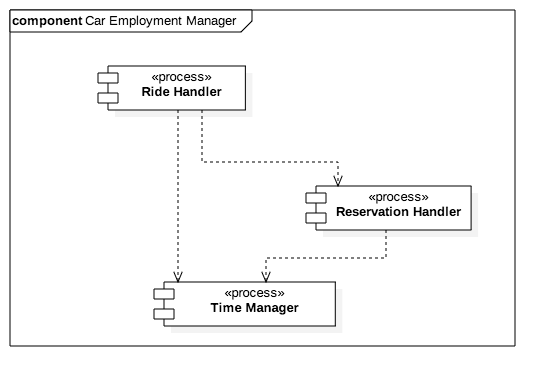
\includegraphics[width=250pt, center]{img/integration_strategy/subcomponents/car_employment_manager.png}
			\end{figure}
		\FloatBarrier

		\paragraphnewline{Money Saving Option}
			\begin{itemize}[label={},leftmargin=*,noitemsep,topsep=0pt]
				\item \textit{Internal integration strategy:} critical-first.
				\item \textit{Integration order:}
					\begin{itemize}[noitemsep]
						\item Parking Distribution Handler
						\item MSO Handler
					\end{itemize}
				\item \textit{Notes: } The Parking Distribution Handler is considered to be the most critical subcomponent between the two, since it has to deal with the core MSO algorithm, moreover exploiting not completely supported tools (as FCL for the fuzzy system).
			\end{itemize}
			\begin{figure}[h]
				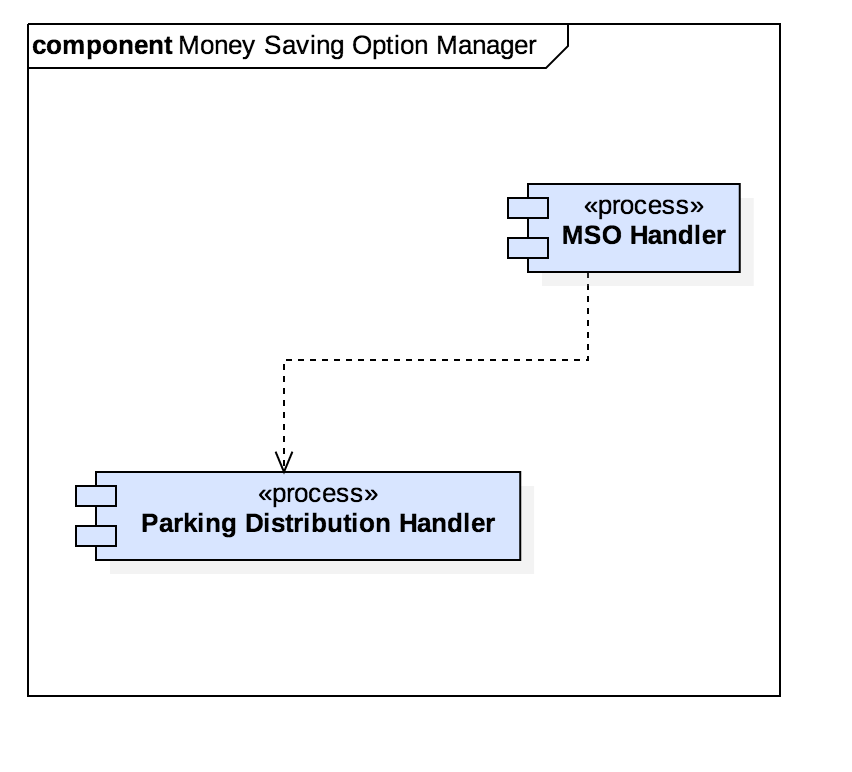
\includegraphics[width=250pt, center]{img/integration_strategy/subcomponents/money_saving_option_manager.png}
			\end{figure}
		\FloatBarrier

		\paragraphnewline{Maintenance Manager}
			\begin{itemize}[label={},leftmargin=*,noitemsep,topsep=0pt]
				\item \textit{Internal integration strategy:} bottom-up.
				\item \textit{Integration order:}
					\begin{itemize}[noitemsep]
						\item Report Status Handler
						\item Emergency Report Handler
						\item Operators Handler
						\item Dispatch Manager
					\end{itemize}
			\end{itemize}
			\begin{figure}[h]
				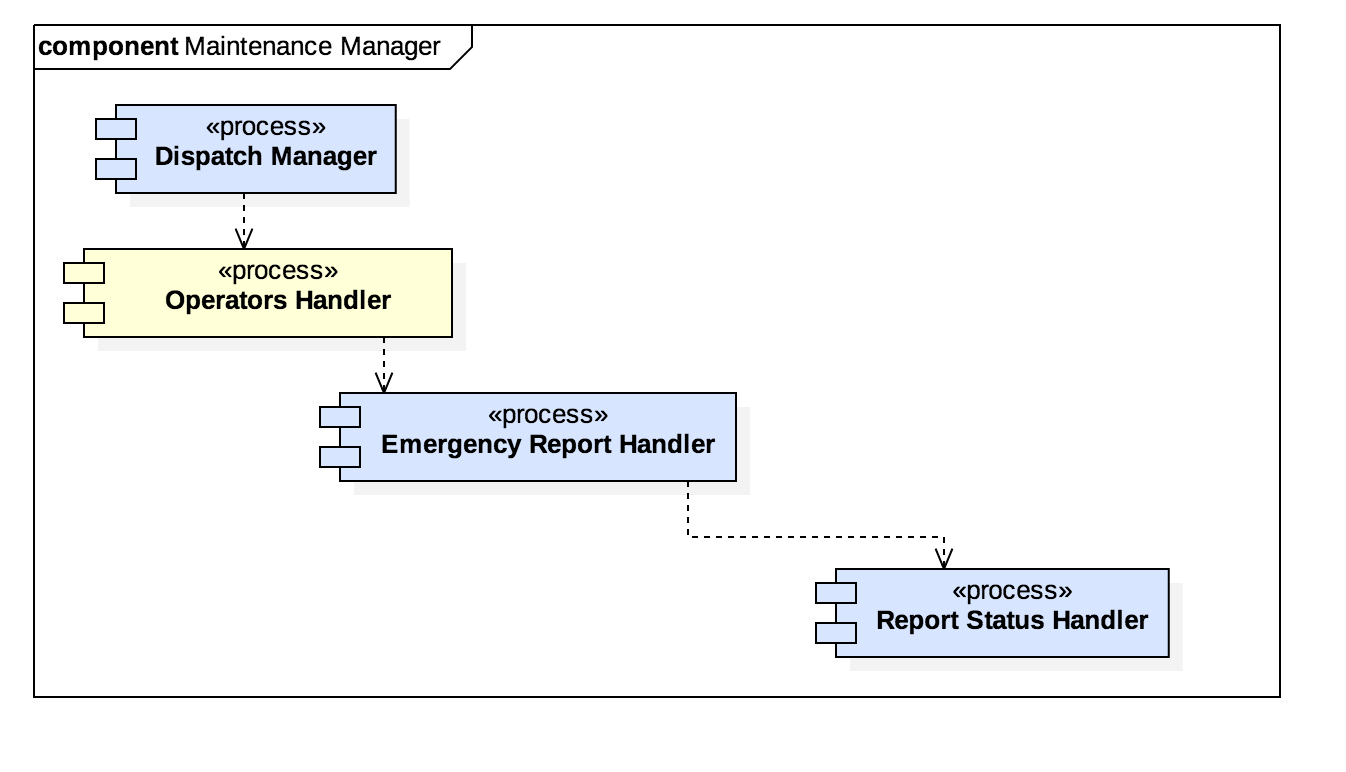
\includegraphics[width=250pt, center]{img/integration_strategy/subcomponents/maintenance_manager.png}
			\end{figure}
		\FloatBarrier

		\paragraphnewline{Payment Manager}
			\begin{itemize}[label={},leftmargin=*,noitemsep,topsep=0pt]
				\item \textit{Internal integration strategy:} critical-first.
				\item \textit{Integration order:}
					\begin{itemize}[noitemsep]
						\item Invoice Manager
						\item Payment Handler
						\item Exceptional Payment Handler
						\item Discount and Sanction Handler
					\end{itemize}
				\item \textit{Notes: } invoice Manager is considered to be the most critical for its responsibility to interact with the external \textit{Payment Services Provider}. The two payment handlers are considered then, and the standard one is privileged because of its importance for the core functioning of the system. Finally the Discount and Sanction Handler is considered to require less effort and is associated to an inferior level of criticality.
			\end{itemize}
			\begin{figure}[h]
				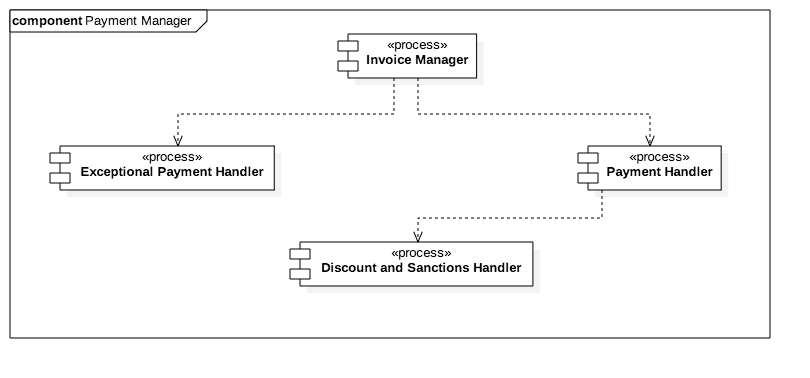
\includegraphics[width=250pt, center]{img/integration_strategy/subcomponents/payment_manager.png}
			\end{figure}
		\FloatBarrier

		\paragraphnewline{Backend Manager}
			\begin{itemize}[label={},leftmargin=*,noitemsep,topsep=0pt]
				\item \textit{Internal integration strategy:} bottom-up.
				\item \textit{Integration order:}
					\begin{itemize}[noitemsep]
						\item Backend Manager
						\item Admin Handler
					\end{itemize}
			\end{itemize}
			\begin{figure}[h]
				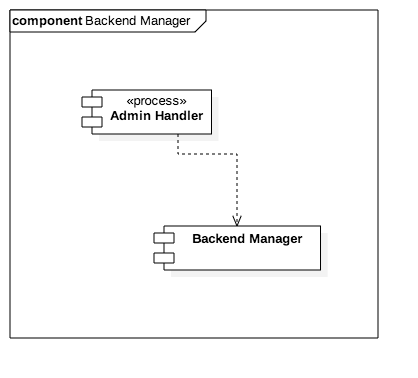
\includegraphics[width=250pt, center]{img/integration_strategy/subcomponents/backend_manager.png}
			\end{figure}
		\FloatBarrier

	\subsubsection{Subsystem integration sequence}
	\label{sec:subsystem_integration_sequence}
		% - list of integration steps for each subsystem until the whole system is completed
		% - images for each level only with components already integrated (progress status)
		% - at the end image with all levels highlighted (in a single image)
		The integration of the macro-components is performed, as said, in a bottom-up fashion. Below are the 5 steps in which this process has been divided for scheduling reasons. Inside a single step, multiple macro-components participate in the integration, each one relying on the macro-components in the previous levels.

		\begin{figure}[h]
			\paragraphnewline{Step 0: Localization Manager}
			The localization manager been developed and unit tested is the starting point for the integration.
			\par\bigskip
			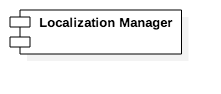
\includegraphics[width=100pt,center]{img/integration_strategy/steps/high_level_components_lv0.png}
			\caption{Subsystem integration sequence: step 0.}
		\end{figure}
		\FloatBarrier

		\begin{figure}[h]
			\paragraphnewline{Step 1: User Manager, Car Manager}
			\par\bigskip
			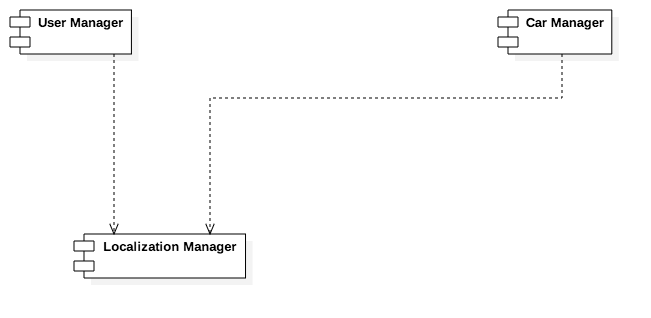
\includegraphics[width=300pt,center]{img/integration_strategy/steps/high_level_components_lv1.png}
			\caption{Subsystem integration sequence: step 1.}
		\end{figure}
		\FloatBarrier

		\begin{figure}[h]
			\paragraphnewline{Step 2: Access Manager, Parking Manager}
			\par\bigskip
			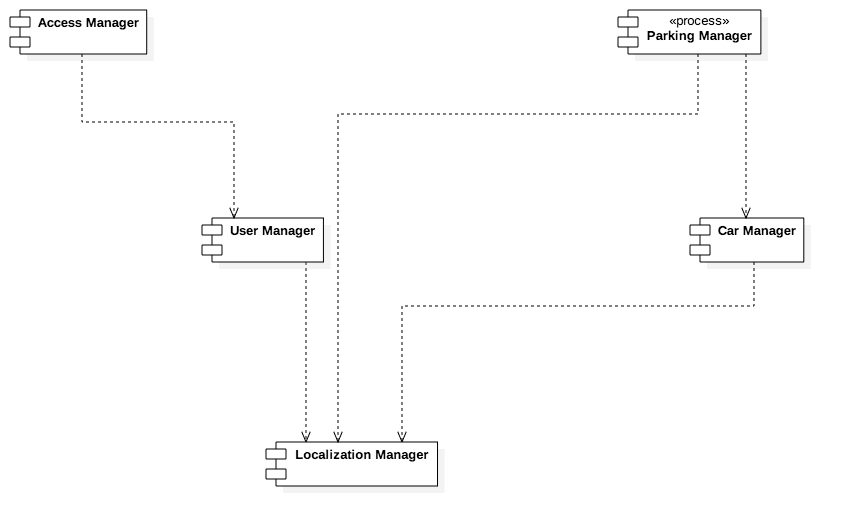
\includegraphics[width=400pt,center]{img/integration_strategy/steps/high_level_components_lv2.png}
			\caption{Subsystem integration sequence: step 2.}
		\end{figure}
		\FloatBarrier

		\begin{figure}[h]
				\paragraphnewline{Step 3: Maintenance Manager, Car Employment Manager, Money Saving Option Manager}
				\par\bigskip
				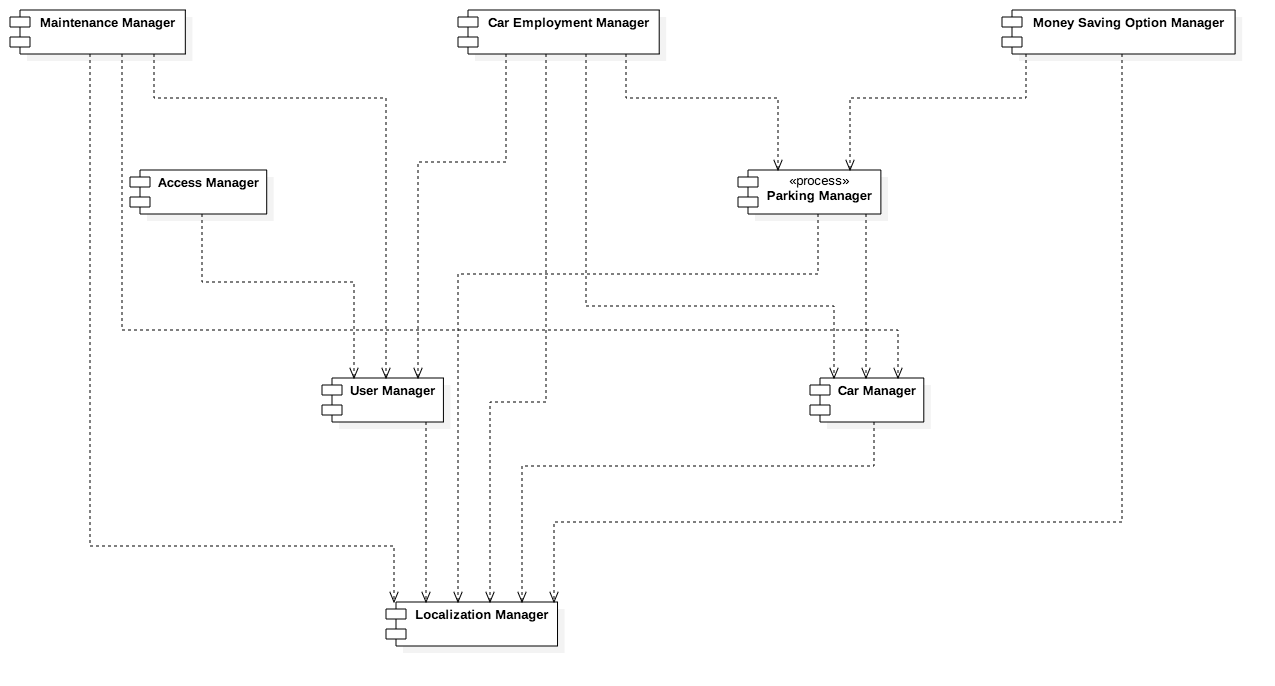
\includegraphics[width=\textwidth,center]{img/integration_strategy/steps/high_level_components_lv3.png}
				\caption{Subsystem integration sequence: step 3.}
			\end{figure}
		\FloatBarrier

		\begin{figure}[h]
			\paragraphnewline{Step 4: Backend Manager, Payment Manager}
			\par\bigskip
			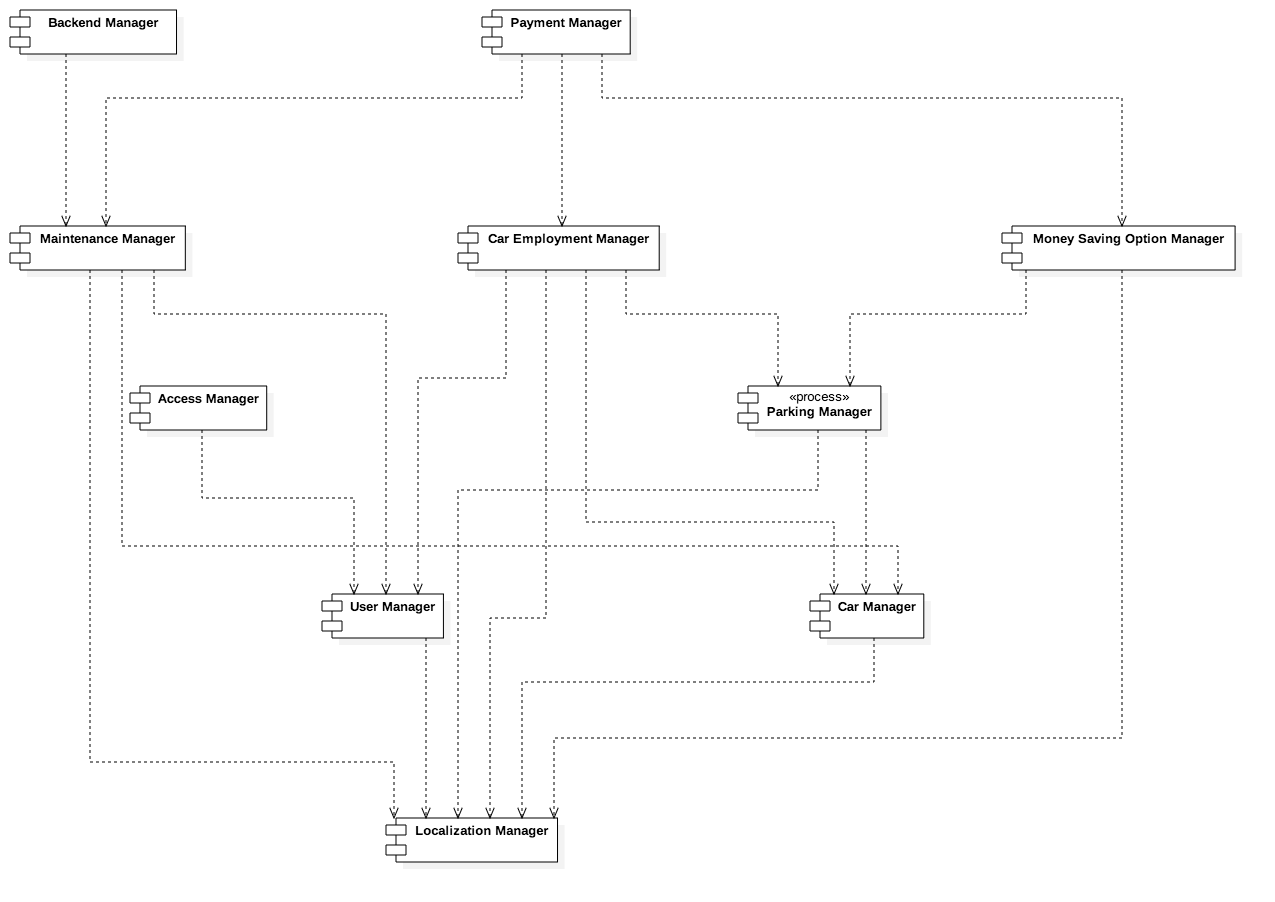
\includegraphics[width=\textwidth,center]{img/integration_strategy/steps/high_level_components_lv4.png}
			\caption{Subsystem integration sequence: step 4.}
		\end{figure}
		\FloatBarrier

		\begin{figure}[h]
			\paragraphnewline{Complete system}
			The complete system integration is summarized in the following image, displaying also the internal structure of each macro-component.
			\par\bigskip
			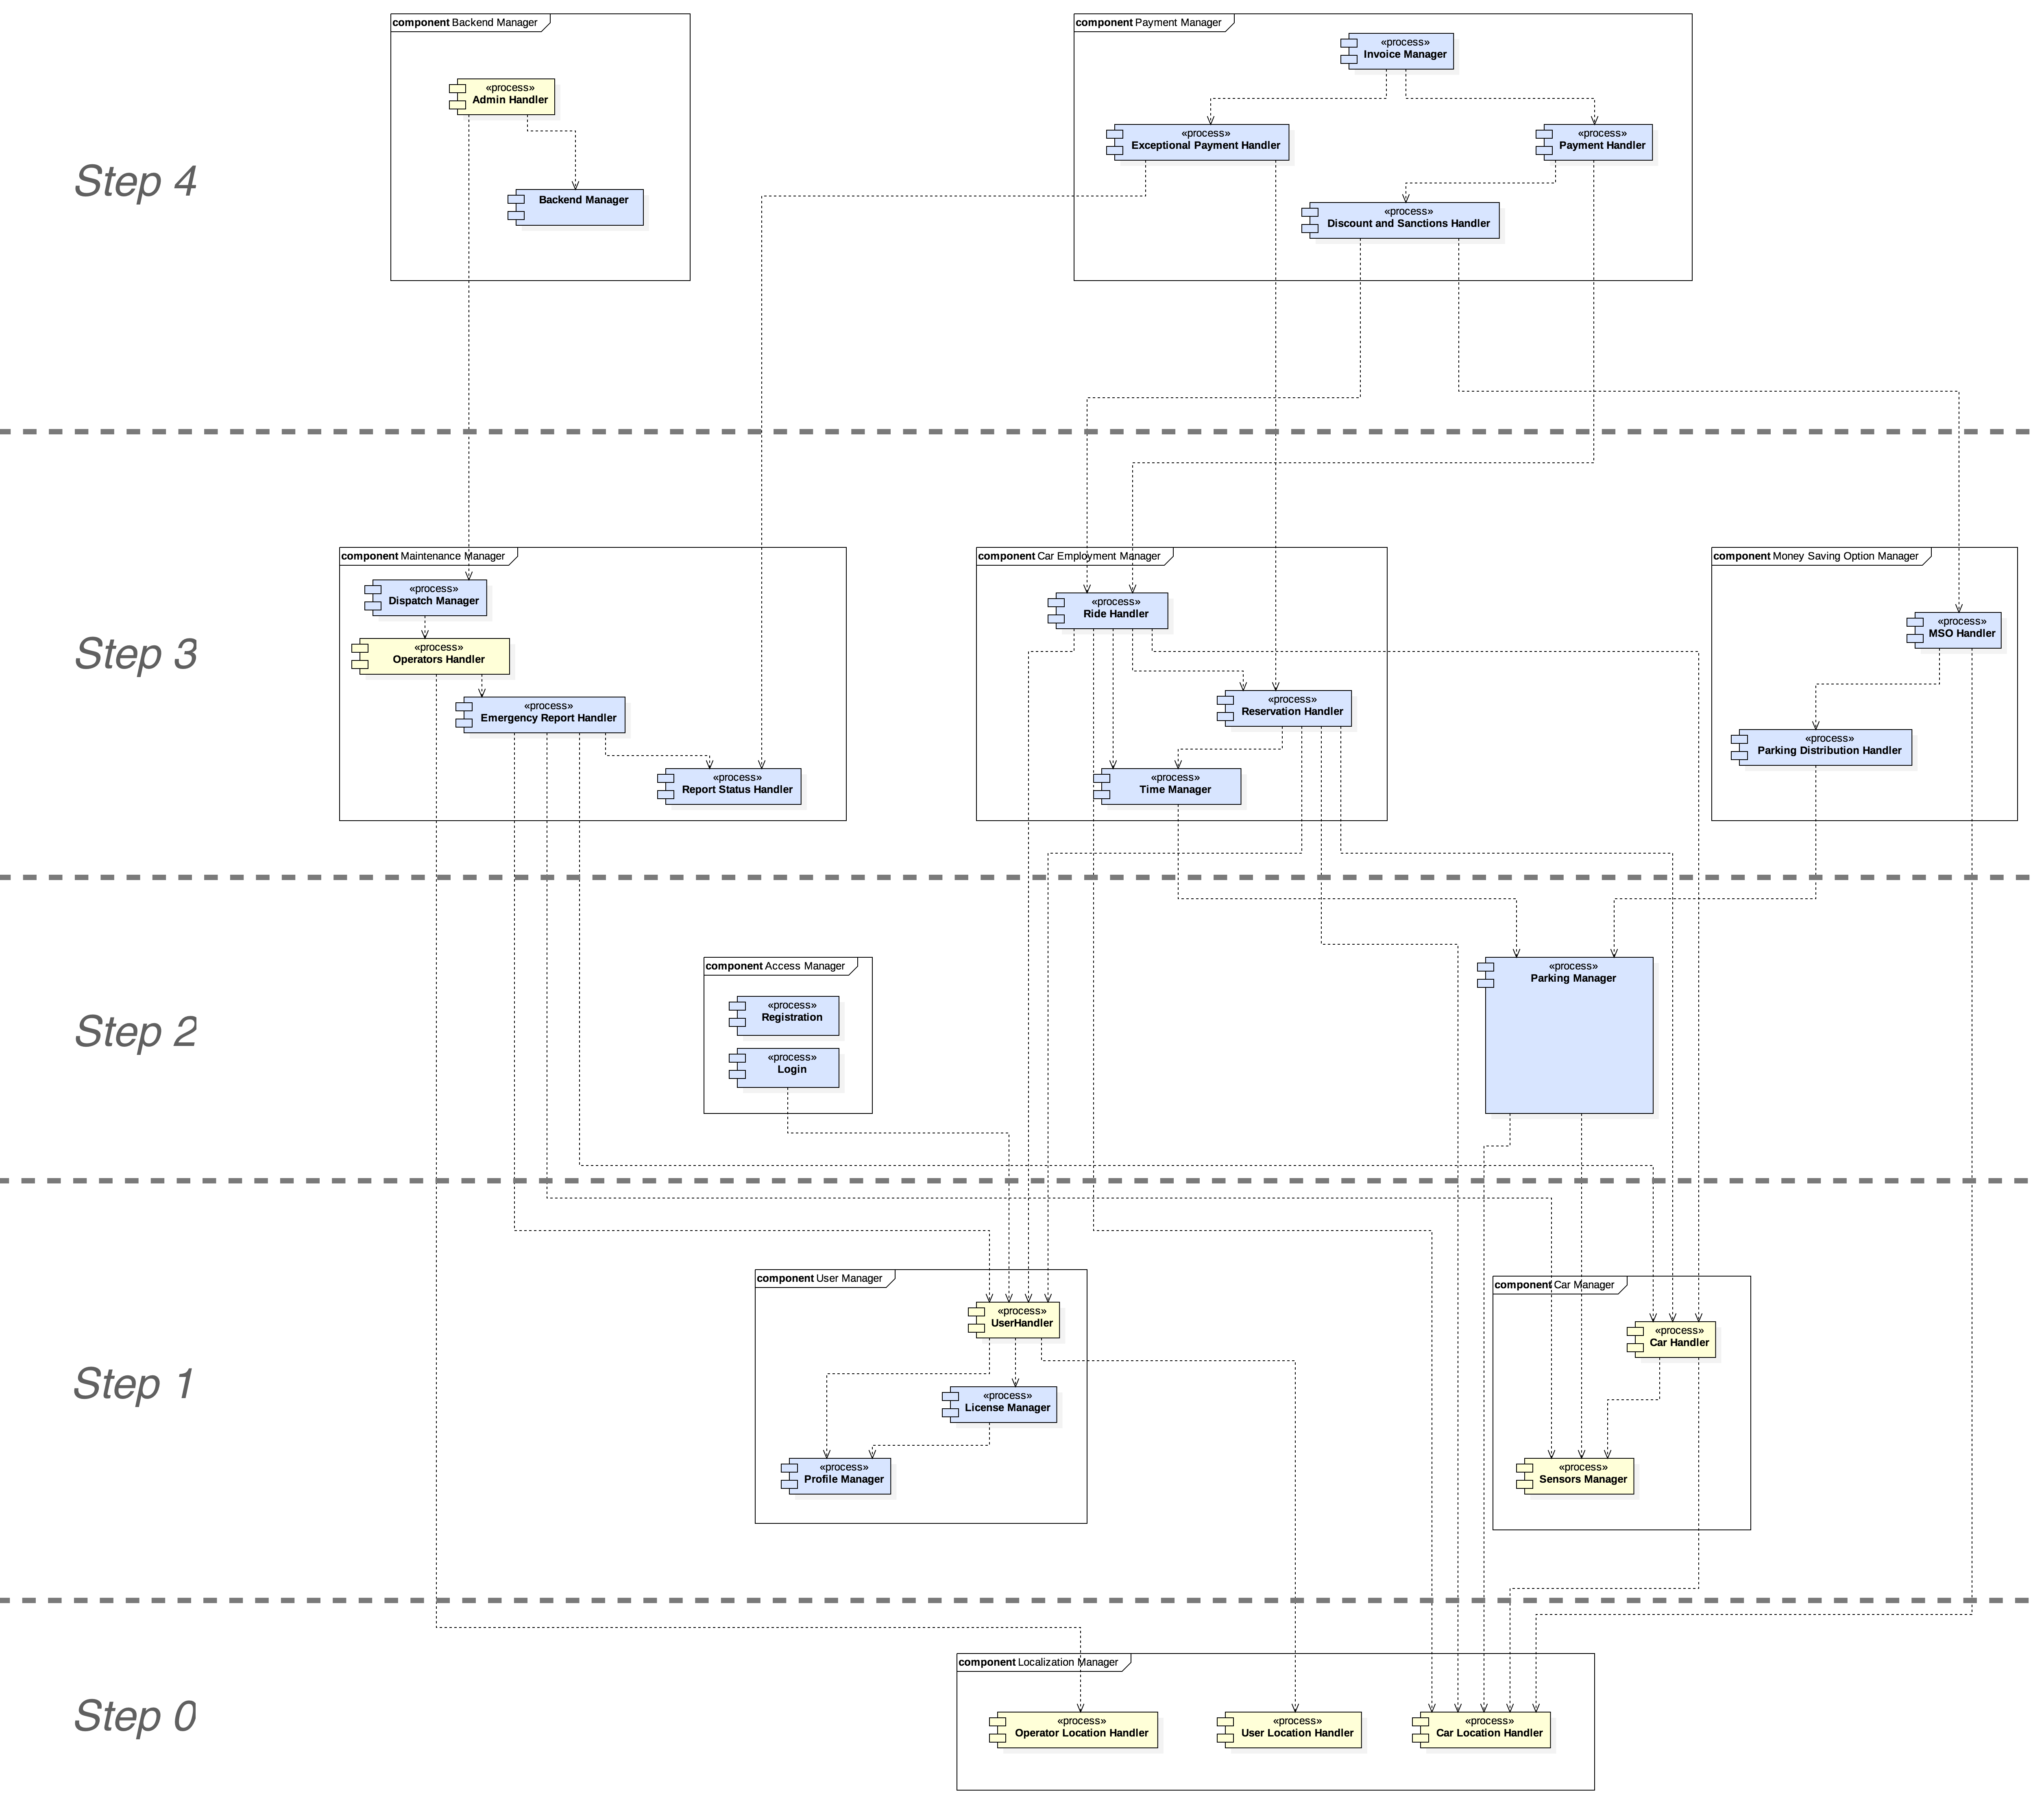
\includegraphics[width=\textwidth,center]{img/integration_strategy/complete_unravelled-steps.png}
			\caption{Complete system and integration steps.}
		\end{figure}
		\FloatBarrier


	\newpage
	\section{Individual steps and test description}
			\label{sec: individual_steps}
	\subsubsection{User Manager}
		\subsubsection*{User Handler, Profile Manager }
			\begin{tabular}{ |l|l| }
				\hline
				\multicolumn{2}{|c|}{CheckData(user: Credentials):bool}\\
				\hline 
				\textit{Input}&\textit{Effect}\\ \hline
				Null parameter & A NullArgumentException is raised\\ \hline
				Right credentials & True\\ \hline
				Wrong credentials & False\\ \hline
			\end{tabular}
			\\
			\begin{tabular}{ |l|l| }
				\hline
				\multicolumn{2}{|c|}{ChangeData(user: Credentials, changedData: Credentials)}\\
				\hline
				\textit{Input}&\textit{Effect}\\ \hline
				Null parameter & A NullArgumentException is raised\\ \hline
				Old credentials and New credentials are the same & An IllegalArgumentException is raised \\ \hline
				New credentials are not valid & An IllegalArgumentException is raised\\ \hline
				New credentials are valid & User's credentials are changed \\ \hline
			\end{tabular}
			\\		
			
		\subsubsection*{User Handler, License Manager}
			\begin{tabular}{ |l|l| }
				\hline
				\multicolumn{2}{|c|}{CheckLicenseValidity(user: Credentials): bool}\\
				\hline
				\textit{Input}&\textit{Effect}\\ \hline
				Null parameter & A NullArgumentException is raised\\ \hline
				Valid driving license & True\\ \hline
				Not valid driving license & False\\ \hline
			\end{tabular}
			\\
			
			\subsubsection*{User Handler, User Location Handler}
			\begin{tabular}{ |l|l| }
				\hline
				\multicolumn{2}{|c|}{SelectZone(location: Location, radius: float)}\\
				\hline
				\textit{Input}&\textit{Effect}\\ \hline
				Null parameter & A NullArgumentException is raised\\ \hline
				Zone selected & Boundaries are defined \\ \hline
			\end{tabular}
			\\
			\begin{tabular}{ |l|l| }
				\hline
				\multicolumn{2}{|c|}{LocateUser(genericUser: Credentials):Location}\\
				\hline
				\textit{Input}&\textit{Effect}\\ \hline
				Null parameter & A NullArgumentException is raised\\ \hline
				Valid parameter  &  Information about User's location \\ \hline
			\end{tabular} 
			\\
			\begin{tabular}{ |l|l| } %TODO
				\hline
				\multicolumn{2}{|c|}{LocateAddress(address: String):Location}\\
				\hline
				\textit{Input}&\textit{Effect}\\ \hline
				Null parameter & \\ \hline
				Valid parameter  &  \\ \hline
			\end{tabular}
			\\
			\subsubsection*{Emergency Report Handler, User Handler}
			\begin{tabular}{ |l|l| }
				\hline
				\multicolumn{2}{|c|}{Notify(command: Command)}\\
				\hline
				\textit{Input}&\textit{Effect}\\ \hline
				Null parameter & A NullArgumentException is raised\\ \hline
				Valid parameter & Notification is recieved \\ \hline
			\end{tabular}
			\\			
			
			\subsubsection*{Reservation Handler, User Handler}
			\begin{tabular}{ |l|l| }
				\hline
				\multicolumn{2}{|c|}{ReserveCar(car: Car)}\\
				\hline
				\textit{Input}&\textit{Effect}\\ \hline
				Null parameter & A NullArgumentException is raised\\ \hline
				Valid parameter & Car is picked for reservation process \\ \hline
			\end{tabular}
			\\
			
			\subsubsection*{Ride Handler, User Handler}
			\begin{tabular}{ |l|l| }
				\hline
				\multicolumn{2}{|c|}{PickupCar(car: Car)}\\
				\hline
				\textit{Input}&\textit{Effect}\\ \hline
				Null parameter & A NullArgumentException is raised\\ \hline
				Valid parameter & The \textit{pickup process} is started \\ \hline
			\end{tabular}
			\\	
			
			\subsubsection*{License Manager, Profile Manager}
			\begin{tabular}{ |l|l| }
				\hline
				\multicolumn{2}{|c|}{CheckData(user: Credentials):bool}\\
				\hline 
				\textit{Input}&\textit{Effect}\\ \hline
				Null parameter & A NullArgumentException is raised\\ \hline
				Right credentials & True\\ \hline
				Wrong credentials & False\\ \hline
			\end{tabular}
			\\
			\begin{tabular}{ |l|l| }
				\hline
				\multicolumn{2}{|c|}{ChangeData(user: Credentials, changedData: Credentials)}\\
				\hline
				\textit{Input}&\textit{Effect}\\ \hline
				Null parameter & A NullArgumentException is raised\\ \hline
				Old credentials and New credentials are the same & An IllegalArgumentException is raised \\ \hline
				New credentials are not valid & An IllegalArgumentException is raised\\ \hline
				New credentials are valid & User's credentials are changed \\ \hline
			\end{tabular}
			\\	
		
		\subsubsection{Car Manager}		
			\subsubsection*{Reservation Handler, Car Handler}
			\begin{tabular}{ |l|l| }
				\hline
				\multicolumn{2}{|c|}{CheckCar():Status}\\
				\hline
				\textit{Input}&\textit{Effect}\\ \hline
				Nothing & Information about car status \\ \hline
			\end{tabular}
			\\
			
			\subsubsection*{Ride Handler, Car Handler}
			\begin{tabular}{ |l|l| }
				\hline
				\multicolumn{2}{|c|}{ChangeState(state: State)}\\
				\hline
				\textit{Input}&\textit{Effect}\\ \hline
				Null parameter & A NullArgumentException is raised\\ \hline
				Valid parameter & The car's state is changed \\ \hline
			\end{tabular}
			\\
			
			\subsubsection*{Car Location Handler, Car Handler} %Changed dependency
			\begin{tabular}{ |l|l| }
				\hline
				\multicolumn{2}{|c|}{NotifyEmergency(signal: Stream)}\\
				\hline
				\textit{Input}&\textit{Effect}\\ \hline
				Null parameter & A NullArgumentException is raised\\ \hline
				Valid parameter &  \\ \hline
			\end{tabular}
			\\		
			
			\subsubsection*{Car Handler, Sensors Manager} 
			\begin{tabular}{ |l|l| }
				\hline
				\multicolumn{2}{|c|}{LockCar()}\\
				\hline
				\textit{Input}&\textit{Effect}\\ \hline
				Null parameter & A NullArgumentException is raised\\ \hline
				Valid parameter & Car is locked  \\ \hline
			\end{tabular}
			\\
			\begin{tabular}{ |l|l| }
				\hline
				\multicolumn{2}{|c|}{UnlockCar()}\\
				\hline
				\textit{Input}&\textit{Effect}\\ \hline
				Null parameter & A NullArgumentException is raised\\ \hline
				Valid parameter & Car is unlocked  \\ \hline
			\end{tabular}
			\\
			\begin{tabular}{ |l|l| }
				\hline
				\multicolumn{2}{|c|}{NotifyIgnition()}\\
				\hline
				\textit{Input}&\textit{Effect}\\ \hline
				Null parameter & A NullArgumentException is raised\\ \hline
				Valid parameter & Notification is recieved  \\ \hline
			\end{tabular}
			\\
			\begin{tabular}{ |l|l| }
				\hline
				\multicolumn{2}{|c|}{NotifyIgnition()}\\
				\hline
				\textit{Input}&\textit{Effect}\\ \hline
				Nothing & Number of detected passengers  \\ \hline
			\end{tabular}
			\\
			
			\subsubsection*{Car Handler, Emergency Report Handler} %Changed dependency
			\begin{tabular}{ |l|l| }
				\hline
				\multicolumn{2}{|c|}{ReportError(error: String)}\\
				\hline
				\textit{Input}&\textit{Effect}\\ \hline
				Null parameter & A NullArgumentException is raised\\ \hline
				Valid parameter &  Error is reported \\ \hline
			\end{tabular}
			\\
			
			
			
			
			
				
			
			
			
			
			
			
			
			
			
			This section contains a detailed description of the tests to be performed on each pair of components that need to be integrated. Those pairs will be identified by a $< caller, called >$ coupled notation that will contain every method called by the $< caller >$ on the $< called >$. 
%	We will follow the bottom-up approach (with partial critical-first approach) as we mentioned in the integration strategy.

	\subsubsection{Employment}
			
		\subsubsection*{Manager, Parking Manager}
		
			\begin{tabular}{ |l|l| }
				\hline
				\multicolumn{2}{|c|}{IsPluggingAllowed(timewindow: Time, curtime: Time, car: Car): bool}\\
				\hline
				\textit{Input} & \textit{Effect}\\ \hline
				One or more null parameters & A NullArgumentException is raised\\ \hline
				$curtime > timewindow$ & False\\ \hline
				$curtime <= timewindow$ & True\\ \hline
			\end{tabular}
			\\
			\begin{tabular}{ |l|l| }
				\hline
				\multicolumn{2}{|c|}{IsParked(car: Car, area: ParkingArea): bool}\\
				\hline
				\textit{Input} & \textit{Effect}\\ \hline
				One or more null parameters & A NullArgumentException is raised\\ \hline
				Car is parked in that safe area & True\\ \hline
				Car is not parked in that safe area & False\\ \hline
			\end{tabular}
			\\			
		
		
		
		\subsubsection*{Ride Handler, Time Manager}
			\begin{tabular}{ |l|l| }
				\hline
				\multicolumn{2}{|c|}{Duration(ride: Ride): Time}\\
				\hline
				\textit{Input} & \textit{Effect}\\ \hline
				Null parameter & A NullArgumentException is raised\\ \hline
				Valid parameter & The time duration of the ride at the time of the request\\ \hline
			\end{tabular}
			\\
		
		
		
		\subsubsection*{Reservation Handler, Time Manager}
			\begin{tabular}{ |l|l| }
				\hline
				\multicolumn{2}{|c|}{SetExpirationTime(time: Time, reservation: Reservation)}\\
				\hline
				\textit{Input} & \textit{Effect}\\ \hline
				One or more null parameters & A NullArgumentException is raised\\ \hline
				The reservation already has an existing expiration time 0& A IllegalArgumentException is raised \\ \hline %FIXIT should it be another exception?
				The reservation doesn't have an expiration time & The expiration time of the reservation is set as $time$\\ \hline
			\end{tabular}
			\\
			\begin{tabular}{ |l|l| }
				\hline
				\multicolumn{2}{|c|}{CheckExpirationTime(reservation: Reservation): bool}\\
				\hline
				\textit{Input} & \textit{Effect}\\ \hline
				Null parameter & A NullArgumentException is raised\\ \hline
				The expiration time for the reservation is still running & True\\ \hline
				The expiration time for the reservation has finished & False\\ \hline
			\end{tabular}
			\\
		
		
		
		\subsubsection*{Ride Handler, Reservation Handler}
			\begin{tabular}{ |l|l| }
				\hline
				\multicolumn{2}{|c|}{CheckReservation(): bool}\\
				\hline
				\textit{Input} & \textit{Effect}\\ \hline
				The reservation is still standing & True\\ \hline
				The reservation is expired & False\\ \hline
			\end{tabular}
			\\
		%TODO not sure this is right: it's not input, there's nothing in input! (also in Exceptional Payment Handler, Reservation Handler)
		
		
		
		\subsubsection*{Discount and Sanctions Handler, Ride Handler}
			\begin{tabular}{ |l|l| }
				\hline
				\multicolumn{2}{|c|}{GetRideInfo(): Ride}\\
				\hline
				\textit{Input} & \textit{Effect}\\ \hline
				Nothing & All the information about the ride\\ \hline
			\end{tabular}
			\\
		
		
		
		\subsubsection*{Payment Handler, Ride Handler}
			\begin{tabular}{ |l|l| }
				\hline
				\multicolumn{2}{|c|}{GetRideInfo(): Ride}\\
				\hline
				\textit{Input} & \textit{Effect}\\ \hline
				Nothing & All the information about the ride\\ \hline
			\end{tabular}
			\\
		
		
		
		\subsubsection*{Parking Distribution Handler, Parking Manager}
			\begin{tabular}{ |l|l| }
				\hline
				\multicolumn{2}{|c|}{GetCars(parkingArea: ParkingArea): List$<Car>$}\\
				\hline
				\textit{Input} & \textit{Effect}\\ \hline
				Null parameter & A NullArgumentException is raised\\ \hline
				Valid input & The list of cars parked in parkingArea\\ \hline
			\end{tabular}
			\\
		
		
		
		\subsubsection*{ExceptionalPaymentHandler, ReservationHandler}
			\begin{tabular}{ |l|l| }
				\hline
				\multicolumn{2}{|c|}{CheckReservation(reservation: Reservation): bool}\\
				\hline
				\textit{Input} & \textit{Effect}\\ \hline
				The reservation is still standing & True\\ \hline
				The reservation is expired & False\\ \hline
			\end{tabular}
			\\
	
	
	
	
	
	\subsubsection{Money Saving Option}
		
		
			
		\subsubsection*{MSO Handler, Parking Distribution Handler}
			\begin{tabular}{ |l|l| }
				\hline
				\multicolumn{2}{|c|}{GetAreas(destination: Location, radius: float): List$<ParkingArea>$}\\
				\hline
				\textit{Input} & \textit{Effect}\\ \hline
				One or more null parameters & A NullArgumentException is raised\\ \hline
				$radius \leq 0$ & A IllegalArgumentException is raised\\ \hline
				Destination outside city boundaries & A IllegalArgumentException is raised\\ \hline
				Valid input & The list of parking areas in a radius around the destination\\ \hline
			\end{tabular}
			\\
		
		
		
		\subsubsection*{Discount and Sanctions Handler, MSO Handler}
			\begin{tabular}{ |l|l| }
				\hline
				\multicolumn{2}{|c|}{CalculateSolution(destination: Location): ParkingArea}\\
				\hline
				\textit{Input} & \textit{Effect}\\ \hline
				Null parameter & A NullArgumentException is raised\\ \hline
				Destination outside city boundaries & A IllegalArgumentException is raised\\ \hline
				Valid input & The parking area where the user should park\\ \hline
			\end{tabular}
			\\
		
	
	
	
	
	\subsubsection{Backend}
	
		\subsubsection*{Operators Handler, Operator Location Handler}
			\begin{tabular}{ |l|l| }
				\hline
				\multicolumn{2}{|c|}{LocateUser(genericUser: Credentials): Location}\\
				\hline
				\textit{Input} & \textit{Effect}\\ \hline
				Null parameter & A NullArgumentException is raised\\ \hline
				Given credentials belong to an Admin or a User & A IllegalArgumentException is raised\\ \hline
				Valid credentials & The location of the Operator\\ \hline
			\end{tabular}
			\\
		
		
		
		\subsubsection*{Dispatch Manager, Operators Handler}
			\begin{tabular}{ |l|l| }
				\hline
				\multicolumn{2}{|c|}{FindOperator(location: Location, radius: float): List$<Operator>$}\\
				\hline
				\textit{Input} & \textit{Effect}\\ \hline
				Null location parameter & A NullArgumentException is raised\\ \hline
				$radius \leq 0$ & A IllegalArgumentException is raised\\ \hline
				Valid parameters & A list of operators in a radius around the location\\ \hline
			\end{tabular}
			\\
			\begin{tabular}{ |l|l| }
				\hline
				\multicolumn{2}{|c|}{CheckAvailability(operator: Credentials): bool}\\
				\hline
				\textit{Input} & \textit{Effect}\\ \hline
				Null parameter & A NullArgumentException is raised\\ \hline
				Given credentials belong to an Admin or a User & A IllegalArgumentException is raised\\ \hline
				Available operator & True\\ \hline
				Unavailable operator & False\\ \hline
			\end{tabular}
			\\
			
		
		
		\subsubsection*{Operators Handler, Emergency Report Handler}
			\begin{tabular}{ |l|l| }
				\hline
				\multicolumn{2}{|c|}{CheckStatus(report: Report): Status}\\
				\hline
				\textit{Input} & \textit{Effect}\\ \hline
				Null parameter & A NullArgumentException is raised\\ \hline
				Valid parameter & The complete status information of the report\\ \hline
			\end{tabular}
			\\
			\begin{tabular}{ |l|l| }
				\hline
				\multicolumn{2}{|c|}{UpdateRecord(report: Report, newStatus: Status)}\\
				\hline
				\textit{Input} & \textit{Effect}\\ \hline
				One or more null parameters & A NullArgumentException is raised\\ \hline
				Valid parameters & The status of the report gets updated\\ \hline
			\end{tabular}
			\\
		
		
		
		\subsubsection*{Emergency Report Handler, Report Status Handler}
			\begin{tabular}{ |l|l| }
				\hline
				\multicolumn{2}{|c|}{CloseReport(report: Report, operator: Credentials)}\\
				\hline
				\textit{Input} & \textit{Effect}\\ \hline
				One or more null parameters & A NullArgumentException is raised\\ \hline
				Given credentials belong to an Admin or a User & A IllegalArgumentException is raised\\ \hline
				The operator is not assigned to the record & A IllegalArgumentException is raised\\ \hline
				Valid parameters & The reports becomes \textit{closed}\\ \hline
			\end{tabular}
			\\
		
		
		
		\subsubsection*{Exceptional Payment Handler, Report Status Handler}
			\begin{tabular}{ |l|l| }
				\hline
				\multicolumn{2}{|c|}{CheckStatus(report: Report): Status}\\
				\hline
				\textit{Input} & \textit{Effect}\\ \hline
				Null parameter & A NullArgumentException is raised\\ \hline
				Valid parameter & The complete status information of the report\\ \hline
			\end{tabular}
			\\
			%TODO add also ChangeStatus for closing reports that require a payment from the user?
		
		
		
		\subsubsection*{Admin Handler, Dispatch Manager}
			\begin{tabular}{ |l|l| }
				\hline
				\multicolumn{2}{|c|}{AssignOperator(report: Report, operator: Credentials}\\
				\hline
				\textit{Input} & \textit{Effect}\\ \hline
				One or more null parameters & A NullArgumentException is raised\\ \hline
				Valid parameters & The operator is assigned to the report\\ \hline
			\end{tabular}
			\\
		
		
		
		\subsubsection*{AdminHandler, Backend Manager}
			\begin{tabular}{ |l|l| }
				\hline
				\multicolumn{2}{|c|}{ChangeParameter(paramToChange: Parameter, newValue: Parameter)}\\
				\hline
				\textit{Input} & \textit{Effect}\\ \hline
				One or more null parameters & A NullArgumentException is raised\\ \hline
				Valid parameters & The new value is assigned to the parameter\\ \hline
			\end{tabular}
			\\
			\begin{tabular}{ |l|l| }
				\hline
				\multicolumn{2}{|c|}{CheckParameter(paramToChange: Parameter, newValue: Parameter): bool}\\
				\hline
				\textit{Input} & \textit{Effect}\\ \hline
				One or more null parameters & A NullArgumentException is raised\\ \hline
				The new value is within the acceptable range for the parameter & True\\ \hline
				The new value is not within the acceptable range for the parameter & False\\ \hline
			\end{tabular}
			\\
			\label{sec: individual_steps_4}
	\subsubsection{Authentication}
		\subsubsection*{Login, User Handler }
			\begin{tabular}{ |l|l| }
				\hline
				\multicolumn{2}{|c|}{Notify()}\\
				\hline 
				\textit{Input}&\textit{Effect}\\ \hline
				Null parameter & A NullArgumentException is raised\\ \hline
				Valid parameter & A notification is sent \\ \hline
			\end{tabular}
			\\
	%TODO login(), signup()
	 \subsubsection{Payment}
		 \subsubsection*{Payment Handler, Discounts and Sanctions Handler }
			\begin{tabular}{ |l|l| }
				\hline
				\multicolumn{2}{|c|}{ApplyDiscounts(discount: float, payment: Payment)}\\
				\hline 
				\textit{Input}&\textit{Effect}\\ \hline
				One or more null parameters & A NullArgumentException is raised\\ \hline
				Valid parameters & Discounts are applied to the payment \\ \hline
			\end{tabular}
			\\
			
		\subsubsection*{Invoice Manager, Payment Handler}
			\begin{tabular}{ |l|l| }
				\hline
				\multicolumn{2}{|c|}{Invoice(paymentService: External Interface, payment: Payment, creditCardInfo: Credentials):bool}\\
				\hline 
				\textit{Input}&\textit{Effect}\\ \hline
				One or more null parameters & A NullArgumentException is raised\\ \hline
				Valid parameters & True \\ \hline
				Not valid parameters & False \\ \hline
			\end{tabular}
			\\
			
		\subsubsection*{Invoice Manager, Exceptional Payment Handler}
			\begin{tabular}{ |l|l| }
				\hline
				\multicolumn{2}{|c|}{AssignFineForReport(fine: float, report: Report)}\\
				\hline 
				\textit{Input}&\textit{Effect}\\ \hline
				One or more null parameters & A NullArgumentException is raised\\ \hline
				Valid parameters & %TODO 
				\\ \hline
			\end{tabular}
			\\
			\begin{tabular}{ |l|l| }
				\hline
				\multicolumn{2}{|c|}{AssignFineForReservation(fine: float, reservation: Reservation)}\\
				\hline 
				\textit{Input}&\textit{Effect}\\ \hline
				One or more null parameters & A NullArgumentException is raised\\ \hline
				Valid parameters & %TODO 
				\\ \hline
			\end{tabular}
			\\	
			
		\subsubsection*{Emergency Report Handler, Report Status Handler}
			\begin{tabular}{ |l|l| }
				\hline
				\multicolumn{2}{|c|}{UpdateRecord(report: Report, newStatus: Status)}\\
				\hline
				\textit{Input} & \textit{Effect}\\ \hline
				One or more null parameters & A NullArgumentException is raised\\ \hline
				Valid parameters & Status of the report is upadated \\ \hline
			\end{tabular}
			\\
			\begin{tabular}{ |l|l| }
				\hline
				\multicolumn{2}{|c|}{CheckStatus(report: Report): Status}\\
				\hline
				\textit{Input} & \textit{Effect}\\ \hline
				Null parameter & A NullArgumentException is raised\\ \hline
				Valid parameter & The status information of the report\\ \hline
			\end{tabular}
			\\	
					
					
			
			
		% TODO

	\newpage
	\section{Tools and test equipment required}
%		\subsection{Tools}
	The testing activities will be performed with the help of various tools, each one designed for a particular task or application domain. In this section, a summary of their capabilities and the ways they are planned to be used is presented. Since they usually are designed to work on a specific platform and/or technology, a distinction will be made on this parameter.

	\subsubsection*{Application Server}
		\begin{itemize}[label={},leftmargin=*,noitemsep,topsep=0pt]
			\item \textit{Technology used} JEE
			\item \textit{Testing tools}
				\begin{itemize}[label={},noitemsep]
					\item \textbf{Mockito} A framework for creating mocks object, useful in integration testing (besides basic unit testing). The mocks can be used to efficiently define stubs to support the scaffolding and test if a component interacts properly with the interfaces on which it depends. In particular, we will use it in the testing of the sub-components integrated with critical-first approach, as exposed in \autoref{sec:stubs}.
					\item \textbf{JUnit} Besides for unit testing, JUnit can be exploited to create drivers not only to test a single component, but also it's integration with the underlying portion of the system. It will be used in fact for every driver specified in \autoref{sec:drivers}.
					\item \textbf{Arquillian} An integration testing framework to execute test cases against the containers of a JEE application. It will be used to verify the correctness of the dependency injections of the components, as well as the injection of the database resources.
					\item \textbf{JMeter} A tool to perform performance analysis on the interconnection of a system's components. In particular, it will be exploited to evaluate the non-functional requirements specified in \textit{section 3.2} of the RASD.
				\end{itemize}
		\end{itemize}

	\subsubsection*{Mobile apps - Android, Car app}
	\label{sec:tools_android_apps}
	\begin{itemize}[label={},leftmargin=*,noitemsep,topsep=0pt]
		\item \textit{Technology used} Java for Android
		\item \textit{Testing tools}
			\begin{itemize}[label={},noitemsep]
				\item \textbf{Android Testing Support Library} A framework that provides a set of APIs for testing Android application, including JUnit 4 and UI tests. It will be used in particular to test the integration of the logic components residing on the client. It should be noted that for all the applications, the components physically deployed on the clients are a small set, since the main application logic is located on the server. For this reason, here the integration testing will not be particularly demanding.
				\item \textbf{Android Device Monitor, Android Studio tools, SDK tools} The performance test will be executed using the set of tools provided by Android Studio and the Android SDK, as the Android Device Monitor.
				\item \textbf{Manual testing} The view of the Android mobile apps will be verified with manual testing. In fact, as explained in \autoref{sec:elements_to_be_integrated}, the testing  will require only simple operations and would not justify the overhead introduced by complicated UI analysis tools.
			\end{itemize}
	\end{itemize}

	\subsubsection*{Mobile apps - iOS}
		\begin{itemize}[label={},leftmargin=*,noitemsep,topsep=0pt]
			\item \textit{Technology used} Objective-C.
			\item \textit{Testing tools}
				\begin{itemize}[label={},noitemsep]
					\item \textbf{Xcode IDE, XCTest, OCmock} The development IDE provides also analysis tools which will be exploited to test the application and analyze its performances. In addition, external tools such as XCTest and OCmock will be used.
					\item \textbf{Manual testing} As for the \textit{Android mobile app}, the view will be manual tested.
				\end{itemize}
		\end{itemize}

	\subsubsection*{Mobile apps - Windows Phone}
		\begin{itemize}[label={},leftmargin=*,noitemsep,topsep=0pt]
			\item \textit{Technology used} C\#.
			\item \textit{Testing tools}
				\begin{itemize}[label={},noitemsep]
					\item \textbf{Visual Studio tools, WindowsPhoneTestFramework, other external tools} The integration testing and performance evaluation will be conducted with the set of tools provided by Microsoft, as well as some external tools such as WindowsPhoneTestFramework. 
					\item \textbf{Manual testing} As for the \textit{Android mobile app}, the view will be manual tested.
				\end{itemize}
		\end{itemize}

	\subsubsection*{Admin application}
		\begin{itemize}[label={},leftmargin=*,noitemsep,topsep=0pt]
			\item \textit{Technology used} JEE.
			\item \textit{Testing tools}
				\begin{itemize}[label={},noitemsep]
					\item \textbf{JUnit} As for the \textit{application server}, Junit will be used to setup the drivers mentioned in \autoref{sec:drivers}.
					\item \textbf{Arquillian} As for the \textit{application server}, Arquillian will be used to verify the the dependency injections system.
					\item \textbf{Manual testing} As for the \textit{Android mobile app}, the view of the Admin application will be verified with manual testing, since the functionalities it provides are very limited.
				\end{itemize}
		\end{itemize}

\subsection{Test equipment}
	% tablet
		% screen size and dpi of all OS (Android diff versions to be taken care)
	% desktop
		% normal computer (PC?)
	% server
		% tools from cloud platform (Amazon, whatever) --> check DD: cloud platform?
	In order to perform the actual tests on an environment similar to the production one, a proper equipment is required. Here is a list of what we plan to use in the integration phase and, more importantly, in the system testing phase.

	\subsection*{Mobile apps}
		The most frequent cause of issues in mobile application is the screen size and density. Therefore, the app must be verified on multiple devices. In particular:
			\begin{itemize}
				\item \textbf{User mobile app} For its criticity, it must be tested on at least one device per screen size: 4.5", 5", 6". If possible, different screen densities must be verified as well.
				\item \textbf{Operator mobile app} Less effort can be allocated here, testing at least on a 5" smartphone and on a 10" tablet, since this app is for internal use only.
				\item \textbf{Car client} Since the cars embed only one type of device, the test should be performed mainly on it. Anyway, from time to time the application should be verified to work with other similar tablets as well, to be prepared for an eventual change of the embedded devices (i.e. for economical reasons, deterioration, etc.).
			\end{itemize}
		To overcome eventual issues related to specific vendors' devices or hardware components, the applications that make use of Bluetooth or GPS must be tested on devices of different brands (in particular for Android).

	\subsection*{Admin application}
		The desktop application can be tested on a desktop similar to the ones used by the administrators. Even if JEE is mostly platform-independent, it is mandatory that the testing is performed on machines running the same OS, to ensure complete compatibility.

	\subsection*{App server}
		Depending on the actual environment on which the app server will run, different testing options are available. In particular, cloud services companies usually provide tools and consoles to manage this aspect.
		In any case, we require that a proper testing environment is set up and made accessible to the developers team to constantly test the application-to-be. The test environment must present the same main characteristics of the production environment (same OS, same JEE implementation, etc.), but may have a more limited amount of resources allocated.

		% TODO

	\newpage
	\section{Program stubs and test data required}
			\subsection{Program Stubs and Drivers}
	
	As we mentioned in \autoref{sec:integration_testing_strategy}, we are going to use a bottom-up approach to integrate and test all macro-components of the system. This means that on the one hand we need a series of drivers to perform the method invocations while the higher-level components still haven't been developed. On the other hand, while it's true that in general we don't need stubs since the lower-level components will have been developed before testing the following level, in \autoref{sec:integration_testing_strategy} we specified that three macro-components needed a critical-first approach: these are the \textbf{Money Saving Option Manager}, the \textbf{Car Manager} and the \textbf{Payment Manager}. In the developing of these components we will start by integrating the most critical subcomponent and then the remaining ones. For these reason, the \textbf{Car Manager} integration and the \textbf{Money Saving Option Manager} integration will require drivers (since their critical component is the most low-level one); on the contrary, the \textbf{Payment Manager} will require the definition of stubs to simulate the potential invoked functions.
	For the specifics of each method invocation performed by the drivers, please refer to \autoref{sec: individual_steps}.
		
		\subsubsection{Stubs}
		\label{sec:stubs}
				
			\begin{itemize}
				\item \textbf{•} %TODO PAYMENT MANAGER
			\end{itemize}
		
		
		\subsubsection{Drivers}
		\label{sec:drivers}

		Here follows a list of drivers needed by the system to perform testing according to our strategy. Following the bottom-up approach, drivers for subcomponents will be provided when needed as well as drivers emulating macrocomponents.
		
		\begin{description}
		\item[Localisation Manager]~\\
			\begin{itemize}
				\item \textbf{Localisation Driver} this testing module will invoke the methods exposed by the \textbf{Localisation Manager} component.
			\end{itemize}
		\item[User Manager]~\\ %TODO
		\item[Car Manager]~\\
			\begin{itemize}
				\item \textbf{Car Handler Driver} this testing module will invoke the methods exposed by the \textbf{Car Handler} subcomponent.
				\item \textbf{Car Manager Driver} this testing module will invoke the methods exposed by the \textbf{Car Manager} component.
			\end{itemize}
		\item[Parking Manager]~\\
			\begin{itemize}
				\item \textbf{Parking Manager Driver} this testing module will invoke the methods exposed by the \textbf{Parking Manager} component.
			\end{itemize}
		\item[Access Manager]~\\ %TODO
		\item[MSO Manager]~\\
			\begin{itemize}
				\item \textbf{Parking Distribution Driver} this testing module will invoke the methods exposed by the \textbf{Parking Distribution Handler} subcomponent.
				\item \textbf{MSO Driver} this testing module will invoke the methods exposed by the \textbf{MSO Manager} component.
			\end{itemize}
		\item[Car Employment Manager]~\\
			\begin{itemize}
				\item \textbf{Time Manager Driver} this testing module will invoke the methods exposed by the \textbf{Time Manager} subcomponent.
				\item \textbf{Reservation Driver} this testing module will invoke the methods exposed by the \textbf{Reservation Handler} subcomponent.
				\item \textbf{Employment Driver} this testing module will invoke the methods exposed by the \textbf{Car Employment Manager} component.
			\end{itemize}
		\item[Maintenance Manager]~\\
			\begin{itemize}
				\item \textbf{Report Status Driver} this testing module will invoke the methods exposed by the \textbf{Report Status Handler} subcomponent.
				\item \textbf{Report Driver} this testing module will invoke the methods exposed by the \textbf{Emergency Report Handler} subcomponent.
				\item \textbf{Operators Driver} this testing module will invoke the methods exposed by the \textbf{Operators Handler} subcomponent.
				\item \textbf{Maintenance Driver} this testing module will invoke the methods exposed by the \textbf{Maintenance Manager} component.
			\end{itemize}	
		\item[BackEnd Manager]~\\
			\begin{itemize}
				\item \textbf{Backend Driver} this testing module will invoke the methods exposed by the \textbf{BackEnd Manager} subcomponent.
			\end{itemize}
		\item[Payment Manager]~\\ %TODO
		\end{description}
		
	
	
	
	\subsection{Test Data}
	
	In order to perform the tests specified in \autoref{sec: individual_steps} we will need a range of test data, both valid and invalid. This chapter will list those data in reference to the specific component (or subsystem) that will need them. %FIXIT subsystem????
	
	
	
		\subsubsection{Employment}
		
		\begin{itemize}
			\item A list of valid and invalid \textbf{Reservations}. The set should contain instances exhibiting the following cases:
				\begin{itemize}
					\item Null object
					\item Null fields
					\item Reservation expired
					\item Starting time for the reservation set in the future
					\item Reservation on a car that is being used
					\item Reservation on a nonexistent car
				\end{itemize}
		\end{itemize}
		
		\begin{itemize}
			\item A list of valid and invalid \textbf{Rides}. The set should contain instances exhibiting the following cases:
				\begin{itemize}
					\item Null object
					\item Null fields
					\item Ride that has already ended
					\item Ride on a car that is already being used
					\item Ride on a nonexistent car
					\item Ride associated with a user already using another car
				\end{itemize}
		\end{itemize}
		
		\begin{itemize}
			\item A list of valid and invalid \textbf{ParkingAreas}. The set should contain instances exhibiting the following cases:
				\begin{itemize}
					\item Null object
					\item Null fields
					\item ParkingAreas containing a car that is located somewhere else
					\item ParkingArea outside city boundaries
					\item ParkingArea with more parked cars than slots
					\item Full ParkingArea
					\item Empty ParkingArea
				\end{itemize}
		\end{itemize}
		
		
		
		\subsubsection{Money Saving Option}
		
		\begin{itemize}
			\item A list of valid and invalid \textbf{destinations}. The set should contain instances exhibiting the following cases:
				\begin{itemize}
					\item Null object
					\item Null fields
					\item Destination is outside city boundaries
					\item Destination has no parking areas within the radius requested by the MSO
					\item Destination doesn't exist
					\item Destination is the car's current location
				\end{itemize}
		\end{itemize}
		
		
		
		\subsubsection{Backend}
		
		\begin{itemize}
			\item A list of valid and invalid \textbf{Parameters}. The set should contain instances exhibiting the following cases:
				\begin{itemize}
					\item Null object
					\item Null fields
					\item Parameter value outside allowed range
				\end{itemize}
		\end{itemize}
		
		\begin{itemize}
			\item A list of valid and invalid \textbf{Emergency Reports}. The set should contain instances exhibiting the following cases:
				\begin{itemize}
					\item Null object
					\item Null fields
					\item Report closed
					\item Report without User assigned
					\item Report without Car assigned
					\item Report without Operator assigned
					\item Report with an available Operator assigned
				\end{itemize}
		\end{itemize}
		% TODO

	\newpage
	\section{Effort spent}
		% TODO
%		\begin{description}
%			\item[Abbud, Patricia] around XX hours of work;
%			\item[Andreoli Andreoni, Maddalena] around XX hours of work;
%			\item[Cudrano, Paolo] around XX hours of work.
%		\end{description}

	\newpage
	\section{Appendix}
	\listoffigures

\end{document}
